\part{Data Governance \& Security}
\begin{frame}
			 \partpage
\end{frame}

\section[Data Governance]{Data Governance}

\begin{frame}
  \frametitle{What is data governance}
  %        \begin{definition}\footnotesize
  %          Data governance is a data management concept concerning the capability that enables an organization to ensure that high data quality exists throughout the complete lifecycle of the data. The key focus areas of data governance include availability, usability, consistency, data integrity and data security and includes establishing processes to ensure effective data management throughout the enterprise such as accountability for the adverse effects of poor data quality and ensuring that the data which an enterprise has can be used by the entire organization.
  %        \footnote[1,frame]{\tiny \href{https://en.wikipedia.org/wiki/Data\_governance}{https://en.wikipedia.org/wiki/Data\_governance}}
  %        \end{definition}
  \begin{itemize}
  \item Defines how data is collected, stored, and used
  \item Defines who can access data, when, and under what conditions
  \item Establishes decision rights
  \item Establishes clear lines of accountability
  \item Gives a voice to all appropriate parties
  \item Provides a mechanism for conflict resolutions involving data
  \end{itemize}
\end{frame}


\begin{frame}
  \frametitle{Goals of data governance @ UH}
  \begin{block}{}
    \href{https://www.hawaii.edu/offices/vp-academic-planning-policy/uh-institutional-data-governance/}{The Data Governance Office at the University of {\hawaii}} creates policies and procedures focused on the privacy and security of data under the University’s care. 
  \end{block}
  \begin{block}{Goals}
  \begin{itemize}
  \item Protect the privacy and security of ``Protected Data''
    \begin{itemize}
    \item All non-public data
    \item Institutional data
    \item Research data
    \end{itemize}
%  \item Produce higher quality data for informed decision making
  \item Promote efficient use of resources
  \item Increase transparency and accountability
  \end{itemize}
  \end{block}
\end{frame}


\subsection{Data Classifications @ UH}
\begin{frame}
  \frametitle{Data Classifications @ UH}
  \vspace{-5pt}
  \makebox[\linewidth][c]{
    \resizebox{\textwidth}{!}{%
      \begin{tabular}{l||p{6cm}||p{6cm}}
      %  \multicolumn{8}{c}{ {\large {\textbf{UH-HPC Resource Summary} } } } \\ 
	\toprule                                                                    
        \thead{\large\textbf{Category}} & \thead{\large\textbf{Definition}} & \thead{\large\textbf{Examples}} \\ 
	\midrule  \midrule %\hline
        \textbf{Public} & Access is not restricted and is subject to open records requests  & Student directory information, employee’s business contact info \\
	\midrule  \midrule %\hline
        \multicolumn{3}{c}{ {\large {\textbf{Protected Data} } } } \\ 
	\midrule  \midrule %\hline
        \textbf{Restricted} & Used for UH business only; will not be distributed to external parties; released externally only under the terms of a written MOA or contract & Student contact information, UH ID number \\
	\midrule  
        \textbf{Sensitive} & Data subject to privacy considerations  & Date of birth, job applicant records, salary/payroll information, most student information \\
	\midrule  
        \textbf{Regulated} & Inadvertent disclosure or inappropriate access requires a breach notification by law or is subject to financial fines & FN or first initial/LN in combination with SSN, driver license number, or bank information; credit card, HIPAA, or financial aid information \\            
    \bottomrule
      \end{tabular}%
    }    }
  \vfill
  \centering
    The \href{https://datagov.intranet.hawaii.edu/dgp/}{Data Governance Process (DGP)} applies to collecting, managing, sharing or using data that can be classified as protected data
\end{frame}  

\section{Regulations}

\begin{frame}
  \frametitle{Regulations}
\begin{block}{}
  The following lists of regulations are not exahustive lists that may apply to your data at the university (personal \& research).
  It is important that you know and understand what regulations the data you are working with is subject to.

\end{block}
\end{frame}

\subsection{Personally Identifiable Information (PII)  \& Financial Regulations}
\begin{frame}
  \frametitle{Regulations}
  \begin{block}{Personally Identifiable Information (PII)  \& Financial Regulations}
    \begin{itemize}
    \item \href{https://studentprivacy.ed.gov/ferpa-regulations}{Family Educational Rights and Privacy Act (FERPA)} [UH Policy \href{https://www.hawaii.edu/policy/?action=viewPolicy\&policySection=ap\&policyChapter=7\&policyNumber=022\&menuView=closed}{AP 7.022}]
      \begin{itemize}
      \item Federal law that protects the privacy of student education records
      \end{itemize}
    
    \item Higher Education Act (HEA)
      \begin{itemize}
      \item Federal law that protects the federal financial aid information
      \end{itemize}
      
    \item \href{https://www.ftc.gov/tips-advice/business-center/privacy-and-security/gramm-leach-bliley-act}{Gramm-Leach-Bliley Act (GLBA)}
      \begin{itemize}
      \item Federal law that requires finanical institutions to explain how they share \& protect customer's data
      \end{itemize}

    \item \href{https://gdpr-info.eu/}{General Data Protection Regulation (GDPR)}
      \begin{itemize}
      \item A European Union (EU) consumer protection law that applies to companies collecting PII as part of delivering goods and services
      \end{itemize}

    \item \href{https://www.hhs.gov/hipaa/for-professionals/security/laws-regulations/index.html}{Health Insurance Portability and Accountability Act (HIPPA}) [UH Policy \href{https://www.hawaii.edu/policy/index.php?action=viewPolicy\&policySection=ep\&policyChapter=2\&policyNumber=217\&menuView=closed}{EP 2.217}]
      \begin{itemize}
      \item Federal law that protects the privacy of health information
        \item \href{https://www.hawaii.edu/infosec/hipaa/}{HIPPA @ UH}
      \end{itemize}
    \end{itemize}  
  \end{block}
\end{frame}  



\subsection{Federal Regulations}
\begin{frame}
  \frametitle{Regulations}
  \vspace{-5pt}
  \begin{block}{Federal Regulations}
    \begin{itemize}
    \item \href{https://csrc.nist.gov/publications/detail/sp/800-171/rev-1/final}{National Institute of Standards and Technology Special Programs (NIST) 800-171}
      \begin{itemize}
      \item Federal Department of Defense (DoD) standards aimed at safeguarding Controlled Unclassified Information (CUI)
      \item May apply to grants from DoD and possibly other federal agencies
      \end{itemize}
    
    \item \href{https://www.hsdl.org/?abstract\&did=461297}{National Industrial Security Program [DoD Directive 5220.22-M]}
      \begin{itemize}
      \item Classified data subject to regulation
      \end{itemize}
      
    \item \href{https://www.pmddtc.state.gov/ddtc_public?id=ddtc_public_portal_itar_landing\#tab-itar}{Export Control \& International Traffic in Arms Regulations (ITAR)}
      \begin{itemize}
      \item Federal regulations that impose access, dissemination or participation restrictions on the use and/or transfer of commodities, technical data, or the provision of services subject to United States (US) export controls for reasons of national security, foreign policy, anti-terrorism or non-proliferation
      \end{itemize}

    \item \href{https://www.bis.doc.gov/index.php/regulations/export-administration-regulations-ear}{Export Administration Regulations (EAR)}
      \begin{itemize}
      \item EAR govern whether a person may export a thing from the U.S., reexport the thing from a foreign country, or transfer a thing from one person to another in a foreign country. The EAR apply to physical things (sometimes referred to as "commodities") as well as technology and software.\footnote{\label{EAR on Wikipedia}\tiny\url{https://en.wikipedia.org/wiki/Export_Administration_Regulations}} 
      \end{itemize}
    \end{itemize}
\end{block}
\end{frame}  


\subsection{State Regulations}
\begin{frame}
  \frametitle{Regulations}
  \vspace{-5pt}
  \begin{block}{State Regulations}
    \begin{itemize}
    \item \href{https://www.capitol.hawaii.gov/hrscurrent/Vol11_Ch0476-0490/HRS0487N/HRS_0487N-.htm}{{\hawaii} Revised Statues (HRS) 487N}
      \begin{itemize}
      \item State law that defines the breach notification to the legislature
      \item Examples: First name or First initial and Last name in combination with at least one of the following
        \begin{itemize}
        \item Social Security Number (SSN)
        \item Driver license or State ID \#
        \item Person's finanical account information
          \end{itemize}
      \end{itemize}
    
    \item \href{https://www.capitol.hawaii.gov/hrscurrent/Vol02_Ch0046-0115/HRS0092F/HRS_0092F-.htm}{Uniform Information Practices Act (UIPA)[HRS Chapter 92F]}
      \begin{itemize}
      \item Governs open records requests
      \end{itemize}
    \end{itemize}
\end{block}
\end{frame}  




\subsection{UH Data Related Policies \& Procedures}
\begin{frame}
  \frametitle{UH Data Related Policies \& Procedures}
  \vspace{-7pt}
\makebox[\linewidth][c]{
    \resizebox{\textwidth}{!}{%                                                                                                                                                                                                                                                       
      \begin{tabular}{l||l}
      %  \multicolumn{8}{c}{ {\large {\textbf{UH-HPC Resource Summary} } } } \\                                                                                                                                                                                                       
        \toprule
        \thead{\large\textbf{Policy}} & \thead{\large\textbf{Description}} \\
        \midrule  \midrule %\hline
        \multicolumn{2}{c}{ {\large {\textbf{Administrative Procedure} } } } \\  
        \midrule \midrule
        \href{https://www.hawaii.edu/policy/?action=viewPolicy\&policySection=ap\&policyChapter=2\&policyNumber=215\&menuView=closed}{\textbf{AP2.215}} & Mandatory Training \& Continuing Education Requirements \\
        \midrule
        \href{https://www.hawaii.edu/policy/?action=viewPolicy\&policySection=ap\&policyChapter=7\&policyNumber=022\&menuView=closed}{\textbf{AP7.022}} & FERPA \\
        \midrule \midrule
        \multicolumn{2}{c}{ {\large {\textbf{Executive Policy} } } } \\  
        \midrule \midrule
        \href{https://www.hawaii.edu/policy/?action=viewPolicy\&policySection=ep\&policyChapter=2\&policyNumber=210\&menuView=closed}{\textbf{EP2.210}} & Use and Management of Information Technology Resources \\
        \midrule
        \href{https://www.hawaii.edu/policy/?action=viewPolicy\&policySection=ep\&policyChapter=2\&policyNumber=213\&menuView=closed}{\textbf{EP2.213}} & System and Campus Wide Electronic Channels for Communicating with Students\\
        \midrule        
        \href{https://www.hawaii.edu/policy/?action=viewPolicy\&policySection=ep\&policyChapter=2\&policyNumber=214\&menuView=closed}{\textbf{EP2.214}} & Data Classification Categories \& Information Security Guidelines \\
        \midrule
        \href{https://www.hawaii.edu/policy/?action=viewPolicy\&policySection=ep\&policyChapter=2\&policyNumber=215\&menuView=closed}{\textbf{EP2.215}} & Institutional Data Governance \\
        \midrule
        \href{https://www.hawaii.edu/policy/?action=viewPolicy\&policySection=ep\&policyChapter=2\&policyNumber=216\&menuView=closed}{\textbf{EP2.216}} & Institutional Records Management \& Electronic Approvals/Signatures (\textit{Pending Approval}) \\
        \midrule
        \href{https://www.hawaii.edu/policy/?action=viewPolicy\&policySection=ep\&policyChapter=2\&policyNumber=217\&menuView=closed}{\textbf{EP2.217}} & HIPPA (\textit{To be Revised}) \\
        \midrule
        \href{https://www.hawaii.edu/policy/?action=viewPolicy\&policySection=ep\&policyChapter=2\&policyNumber=218\&menuView=closed}{\textbf{EP2.218}} & Online Approvals of Internal University Transactions\\
        \midrule
        \textbf{EP2.2xx} & Student Online Data Protection Requirements (\textit{Draft}) \\
        \midrule
        \href{https://www.hawaii.edu/policy/?action=viewPolicy\&policySection=ep\&policyChapter=2\&policyNumber=215\&menuView=closed}{\textbf{EP2.215}} & Institutional Data Governance \\
        \midrule
        \href{https://www.hawaii.edu/policy/?action=viewPolicy\&policySection=ep\&policyChapter=8\&policyNumber=200\&menuView=closed}{\textbf{EP8.200}} & Policy on Contracts \& Signing Authority \\
        \bottomrule
      \end{tabular}%
      }
}
\vspace{-5pt}


\end{frame}  



\section[Security]{Security}


\subsection{Information Security Program}
\begin{frame}
  \frametitle{Information Security Program}

  The \href{https://www.hawaii.edu/infosec/infosecprogram/}{University of {\hawaii} Information Security Program} is comprised of the following strategic areas:

  \begin{block}{Strategic Areas}
    \begin{itemize}
  \item Data Governance \& Oversight
  \item Information Security Audits \& Risk Assessments
  \item Information Security Policies \& Procedures
  \item Identity Management \& Access Controls
  \item Information Security Training \& Awareness
  \end{itemize}
  \end{block}
\end{frame}  


\subsection{Data Protection}
\begin{frame}
  \frametitle{Protect Your Data!}
  \vspace{-10pt}
  \begin{block}{Know which files have sensitive information}
    \begin{itemize}
    \item Use \href{http://www.hawaii.edu/askus/1297}{Spirion} (formerly Identity Finder) to scan for sensitive information
    \end{itemize}
  \end{block}
  \vspace{-3pt}  
  \begin{block}{Protect sensitive/regulated data as required by UH policy}
  \begin{itemize}
  \item UH Policy \href{https://www.hawaii.edu/policy/EP2.214}{EP 2.214}
  \end{itemize}
  \end{block}
  \vspace{-3pt}  
  \begin{block}{Data protection life cycle}
    \begin{itemize}
    \item Back up your data regularly
    \item Transmit and share sensitive data in a secure manner, e.g., SFTP, \href{https://www.hawaii.edu/filedrop/}{UH FileDrop}
    \item Protect sensitive/regulared data with encryption
    \item Securely delete any sensitive data that is no longer needed
    \end{itemize}
  \end{block}    
  \vspace{-3pt}  
  \begin{block}{Physical Security of data repository with sensitive data}
    \begin{itemize}
    \item Paper documents should be stored in a secured location, not accessible by unauthorized individuals e.g., a locked file cabinent
    \item External hard drives should be stored in a secured location e.g., a locked file cabinent
    \end{itemize}
  \end{block}    
\end{frame}  

\subsection{Device Protection}
\begin{frame}
  \frametitle{Protect Your Computers!}
  \begin{block}{Operating System (OS) }
    \begin{itemize}
    \item Apply updates to your OS and applications frequently and on a regular basis
    \end{itemize}
  \end{block}

  \begin{block}{Protective Software}
  \begin{itemize}
  \item Install and keep up to date protective software such as \href{http://www.hawaii.edu/askus/1254}{anti-virus}
  \end{itemize}
  \end{block}

  \begin{block}{Physical Access}
    \begin{itemize}
    \item Never leave your devices logged-in \& unattended
    \item Control physical access to your machines
    \item When you step away from your machine, lock your screen
    \item Require password authentication when unlocking or accessing your machine
    \end{itemize}
  \end{block}    
\end{frame}  


\subsection{Storing and transmitting data with Google products}
\begin{frame}
  \frametitle{Storing and transmitting data with Google products}
  \onslide<1->{\begin{block}{Question}
    \begin{columns}[T ]
      \begin{column}{0.15\textwidth}\hfill
\includegraphics[scale=0.05]{question_mark.png}\end{column}
      \begin{column}{0.80\textwidth}
        Is it safe to store and transmit sensitive or regulated data using the different Google products offerred at the University?
        e.g., Google Docs, Google Drive, Gmail
      \end{column}
    \end{columns}
    \end{block}
    }
  \vfill
  \onslide<2->{\begin{block}{Answer}
%https://www.kissclipart.com/stop-hand-clipart-stop-sign-clip-art-pgay2w/
\begin{columns}
\begin{column}{0.15\textwidth}\hfill\includegraphics[scale=0.05]{stop_hand.png}\end{column}
\begin{column}{0.70\textwidth}
    \centering
    {\HUGE \textbf{\textit{NO!}}}\Large~\\Do \textbf{NOT} store or transmit sensitive or regulated information in \emph{Google Docs}, \emph{Google Drive} or \emph{Email}~\\~\\Use the \href{https://www.hawaii.edu/filedrop/}{UH FileDrop} to securely transmit files under 1000 megabytes inside
\end{column}
\begin{column}{0.15\textwidth}\includegraphics[scale=0.05]{stop_hand.png}\end{column}
\end{columns}
    \end{block}}
\end{frame}



\subsection{Account protection}
\begin{frame}
  \frametitle{Protect Your Account!}
\begin{columns}
\begin{column}{0.45\textwidth}
\begin{block}{}
  \begin{itemize}
  \item User strong passwords and a strong password management strategy
  \item \textbf{DO NOT RE-USE PASSWORDS!}
  \item Consider using a passphrase
    \begin{itemize}
    \item lower/uppercase
    \item numbers
    \item special characters
    \item character substitutions, e.g.,
      \begin{itemize}
      \item o $\Longrightarrow$ 0
      \item a $\Longrightarrow$ @
      \item i $\Longrightarrow$ 1
      \end{itemize}
    \end{itemize}
  \item Check your password strength: \href{https://lastpass.com/howsecure.php}{https://lastpass.com/howsecure.php}
  \item Monitor your accounts for suspicious activity
  \end{itemize}
  \end{block}
\end{column}
\begin{column}{0.49\textwidth}
\begin{block}{}
  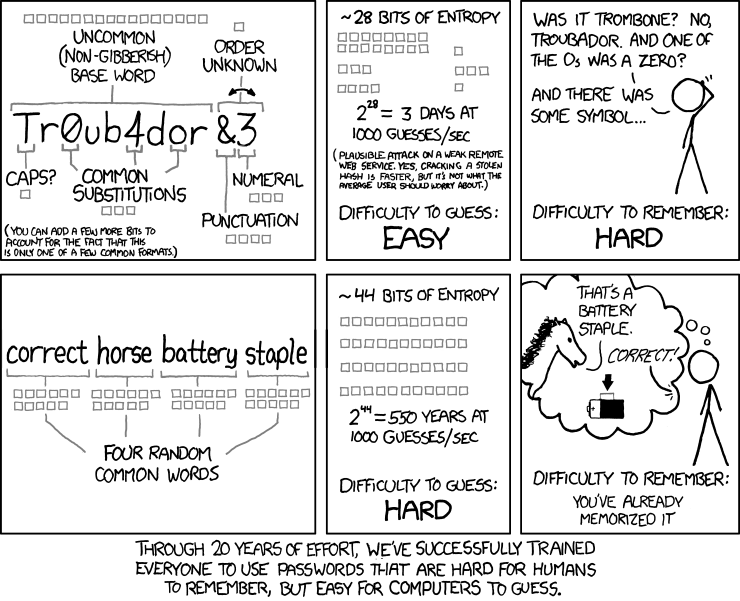
\includegraphics[scale=0.25]{password_strength.png}
  \numlessfootnotetxt{\label{xkcd_pasword_strnght}\tiny\url{https://xkcd.com/936/}}
\end{block}
\end{column}
\end{columns}
\end{frame}  


\section*{More Information}
\begin{frame}
  \frametitle{More Information}
  You can find more information about Data Governance and Security at UH at the following links:
  \begin{itemize}
  \item \href{https://datagov.intranet.hawaii.edu/}{Data Governance internal site}
  \item \href{https://datagov.intranet.hawaii.edu/training/}{Data Governance \& Security trainings/presentations}
  \item \href{https://datagov.intranet.hawaii.edu/institutional-data-classification-levels/}{Institutional data classifications}
  \item \href{https://www.hawaii.edu/infosec/}{Information Security (InfoSec) at UH}
  \item \href{https://www.hawaii.edu/its/alerts/}{Security notices and other alerts from UH Information Technology Services (ITS)}
  \item \href{https://www.hawaii.edu/its/itacw/}{IT All Campus Workshop \ddash Yearly during the summer}
  \end{itemize}
\end{frame}  




  %% \item General Data Protection Regulation (GDPR)
  %%   \begin{itemize}
  %%   \item A European Union (EU) consumer protection law that applies to companies collecting personally identifiable information (PII) as part of delivering goods and services
  %%   \end{itemize}

  %% \item General Data Protection Regulation (GDPR)
  %%   \begin{itemize}
  %%   \item A European Union (EU) consumer protection law that applies to companies collecting personally identifiable information (PII) as part of delivering goods and services
  %%   \end{itemize}

  %% \item General Data Protection Regulation (GDPR)
  %%   \begin{itemize}
  %%   \item A European Union (EU) consumer protection law that applies to companies collecting personally identifiable information (PII) as part of delivering goods and services
  %%   \end{itemize}

  %% \item General Data Protection Regulation (GDPR)
  %%   \begin{itemize}
  %%   \item A European Union (EU) consumer protection law that applies to companies collecting personally identifiable information (PII) as part of delivering goods and services
  %%   \end{itemize}

    
  %% \end{itemize}
  
  %% \begin{table}
  %%   \centering
  %%   \resizebox{\textwidth}{!}{%
  %%     \begin{tabular}{l||p{6cm}||p{6cm}}
  %%     %  \multicolumn{8}{c}{ {\large {\textbf{UH-HPC Resource Summary} } } } \\ 
  %%       \toprule                                                                    
  %%       \thead{\large\textbf{Regulation}} & \thead{\large\textbf{Description}} & \thead{\large\textbf{}} \\ 
  %%       \midrule  \midrule %\hline
  %%       \textbf{Public} & Access is not restricted and is subject to open records requests  & Student directory information, employee’s business contact info \\
  %%       \midrule  \midrule %\hline
  %%       \multicolumn{3}{c}{ {\large {\textbf{Protected Data} } } } \\ 
  %%       \midrule  \midrule %\hline
  %%       \textbf{Restricted} & Used for UH business only; will not be distributed to external parties; released externally only under the terms of a written MOA or contract & Student contact information, UH ID number \\
  %%       \midrule  
  %%       \textbf{Sensitive} & Data subject to privacy considerations  & Date of birth, job applicant records, salary/payroll information, most student information \\
  %%       \midrule  
  %%       \textbf{Regulated} & Inadvertent disclosure or inappropriate access requires a breach notification by law or is subject to financial fines & FN or first initial/LN in combination with SSN, driver license number, or bank information; credit card, HIPAA, or financial aid information \\            
  %%   \bottomrule
  %%     \end{tabular}%
  %%   }
  %% \end{table}


%% \begin{columns}
	%% \begin{column}{0.46\textwidth}
	%% 	\begin{block}{}
	%% 	\begin{itemize}
	%% 		\item Quad Data Rate (QDR)\\InfiniBand{\regtrademark} (IB)   
	%% 			\begin{itemize}
	%% 				\item 40 Gbit
	%% 				\item Older compute nodes
	%% 				\item low latency ($\approx1.3\mu$s)
	%% 				\item non-blocking
	%% 			\end{itemize}
	%% 			~\\
	%% 		\item 25/100 Gbit Ethernet
	%% 			\begin{itemize}
	%% 				\item Newer compute nodes
	%% 				\item Nodes connected @ 25~Gbit
	%% 				\item non-blocking
	%% 			\end{itemize}
	%%         \end{itemize}
        %%         \end{block}
	%% \end{column}
	%% \begin{column}{0.46\textwidth}
	%% 	\begin{block}{External Networks}
	%% 	\begin{itemize}
	%% 		\item 100 Gbit SciDMZ
	%% 			\begin{itemize}
	%% 				\item Login \& compute nodes\\connected via a firewall
	%% 				\item DTNs are directly connected
	%% 			\end{itemize}
	%% 	\end{itemize}
        %%         \end{block}
	%% \end{column}
	%% \end{columns}


        



%% \begin{frame}
%% 	\frametitle{Terminology}
%% 	\begin{itemize}
%% 	\item \textbf{Symbolic Link (symlink)} -- A file that contains a reference to another file or directory
%% 	\item \textbf{Command-line interface/interpreter (CLI)} -- A text-based user interface used to view and manage computer files 
%% 	\item \textbf{Message Passing Interface (MPI)} -- A standard that is used by programs to pass messages between nodes
%% 	\item \textbf{High Performance Compute (HPC)} -- A computing paradigm in which applications are typically a tightly coupled parallel job that benefit from a low-latency interconnect
%% 	\item \textbf{High Throughput Compute (HTC)} -- A computing paradigm that focuses on the efficient execution of a large number of loosely-coupled tasks
%%         \item \textbf{Modified time} -- The last time the file was modified (content has been modified)\footnote{\label{Types of timestamps}\tiny\url{https://unix.stackexchange.com/a/2465}}
%%         \item \textbf{Shell script (script)} -- A computer program designed to be run by a CLI\footnote{\label{Shell script}\tiny\url{https://en.wikipedia.org/wiki/Shell_script}}
%% %        \item Pleasantly Parallel -- Processes are independent and no communication is necessary 
%% 	\end{itemize}


%% \end{frame}


%% \section[University of Hawai'i High Performance Compute Cluster]{University of Hawai'i High Performance Compute Cluster}
%% \begin{frame}
%%     \frametitle{University of {\hawaii} High Performance Compute Cluster}
%%     \begin{itemize}
%%     \item The University~of~{\hawaii} High Performance Compute Cluster~({\uhhpc}) is \textbf{free} to use for all active faculty, staff, and students affiliated with the University of {\hawaii}
%%     \item Community acquired nodes are equally accessible to all users
%%     \item Nodes purchased through the {\textbf{condo program}} are shared with the community, but priority is given to the node owner and their agents
%% 		\item Nodes may be {\textbf{leased}} from the community pool
%% 		\item Additional permanent storage can be leased with up to a five year contract by faculty \& staff
%%     \end{itemize}
%% 		\begin{block}{UH-HPC Resource Summary}
%%   \begin{table}
%%     \centering
%%     \resizebox{\textwidth}{!}{%
%%       \begin{tabular}{l||l||l||l||l||l||l||l}
%%       %  \multicolumn{8}{c}{ {\large {\textbf{UH-HPC Resource Summary} } } } \\ 
%% 			\toprule                                                                    

%%               {}               & \thead{\textbf{Nodes}} & \thead{\textbf{CPU Cores}} & \thead{\textbf{Memory}} & \thead{\textbf{GPUs}} & \thead{\textbf{Home/Group Space}} & \thead{\textbf{Scratch Space}} & Storage for lease \\ 
%% 							\midrule  \midrule %\hline
%%         \thead{\textbf{Total}} & 297                    & 6,308                      & 50 TB                   &  56                   & 80 TB                             &  700 TB                        & 1 PB              \\ %\hline
%% 				\bottomrule
%%       \end{tabular}%
%%     }
%%   \end{table}
%% 	\end{block}
%% \end{frame}

%% \subsection{Condo Program \& Leasing}
%% \begin{frame}
%%   \frametitle{What is the Condo Program \& leasing?}
%% 	\begin{block}{Condo Program}\scriptsize
%% 		\begin{itemize}
%% 		\item The condo program allows faculty \& staff to purchase nodes and have them integrated with the UH-HPC
%% 		\item Condo nodes can take advantage of networking and storage infrastructure that one may not typically have access to
%% 		\item Condo nodes are managed and maintained by ITS staff
%% 		\item No maintenance fee will be assessed until the node is off warranty (typically five years)
%% 		\end{itemize}
%% 	\end{block}
%% 	\begin{block}{Leasing}\scriptsize
%% 		\begin{itemize}
%% 		\item Nodes leased from the community can have a contract period from one month, up to one year
%% 		\item Node lessees are provided priority access to their leased hardware
%% 		\item Leases are not considered an equipment purchase
%% 		\end{itemize}
%% 	\end{block}
%% \end{frame}

%% \subsection{Storage}
%% \begin{frame}
%%   \frametitle{Storage}
%%   The UH-HPC has two classes and three types of storage that users can potentially access.\\Each type of storage has their own attributes and restrictions
%% 	\begin{columns}
%% 		\begin{column}{0.46\textwidth}
%% 		\begin{block}{Free Storage}
%% 			\begin{enumerate}
%% 			\item Permanent Storage
%% 				\begin{itemize}
%% 				\item Home Storage
%% 				\item Group/Lab Storage
%% 				\end{itemize}
%% 			\item Scratch Storage
%% 				\begin{itemize}
%% %				\item {\lustre}(TBD)
%% 				\item Network File System (NFS)
%% 				\end{itemize}
%% 		\end{enumerate}
%% 		\end{block}
%% 		\end{column}
%% 		\begin{column}{0.46\textwidth}
%% 		\begin{block}{For Fee Storage}
%% 			\begin{enumerate}
%% 				\item Long Term Storage (LTS)
%% 		\end{enumerate}
%% 		\end{block}
%% 		\end{column}
%% 	\end{columns}      
%% \end{frame}

%% \begin{frame}
%%   \frametitle{Permanent Storage}
%%   \begin{enumerate}
%%   \item Home Storage
%%     \begin{itemize}
%%     \item {\textbf{Purpose}}: Personal storage for applications and active data that needs to persist on the UH-HPC
%%     \end{itemize}
%%   \item Group/Lab Storage
%%     \begin{itemize}
%%     \item {\textbf{Purpose}}: Group/Lab storage allows users to share data \& applications with a need for persistence on the UH-HPC
%%     \end{itemize}
%%   \end{enumerate}
%% ~\\
%%   All permanent storage options on the UH-HPC have the following attributes:
%%   \begin{itemize}
%%   \item 50 GB default quota with a max quota of 300 GB
%%   \item Quota increases are re-evaluated annually
%%   \item Available on all nodes
%%   \item Freely available to users
%%   \end{itemize}

%% \end{frame}


%% \begin{frame}
%%   \frametitle{Scratch Storage}
%%   \begin{enumerate}
%% %    \item {\lustre (TBD)}
%% %      \begin{itemize}
%% %      \item High performance parallel file system 
%% %      \item 50 TB quota
%% %      \end{itemize}
%%     \item NFS
%%       \begin{itemize}
%% %      \item Not a parallel file system
%%       \item 5 TB quota
%%       \end{itemize}
%%   \end{enumerate}
%% ~\\
%%   All scratch file systems on the UH-HPC have the following attributes:
%%   \begin{itemize}
%%   \item \textbf{Purge policy} -- 10 days based on file modify time
%%   \item Available on all nodes
%%   \item Freely available to users
%%   \end{itemize}

%% \end{frame}



%% %\begin{frame}
%%   %\frametitle{For Fee Storage}
%%   %\begin{enumerate}
%%     %\item ValueStorage
%%       %\begin{itemize}
%%       %\item Enterprise class equipment 
%%       %\item 10 Gbit connected to the UH-HPC
%%       %\item Currently only accessible on the DTNs and login nodes
%%       %\end{itemize}
%%     %\item LTS  
%%       %\begin{itemize}
%%       %\item Cheap-n-Deep
%%       %\item 100 Gbit connected to the UH-HPC
%%       %\item Accessible on all nodes
%%       %\end{itemize}
%%   %\end{enumerate}
%% %\end{frame}



%% \subsection{Networking}
%% \begin{frame}
%%   \frametitle{Networking}
%% 	\begin{columns}
%% 	\begin{column}{0.46\textwidth}
%% 		\begin{block}{Internal Networks}
%% 		\begin{itemize}
%% 			\item Quad Data Rate (QDR)\\InfiniBand{\regtrademark} (IB)   
%% 				\begin{itemize}
%% 					\item 40 Gbit
%% 					\item Older compute nodes
%% 					\item low latency ($\approx1.3\mu$s)
%% 					\item non-blocking
%% 				\end{itemize}
%% 				~\\
%% 			\item 25/100 Gbit Ethernet
%% 				\begin{itemize}
%% 					\item Newer compute nodes
%% 					\item Nodes connected @ 25~Gbit
%% 					\item non-blocking
%% 				\end{itemize}
%% 	        \end{itemize}
%%                 \end{block}
%% 	\end{column}
%% 	\begin{column}{0.46\textwidth}
%% 		\begin{block}{External Networks}
%% 		\begin{itemize}
%% 			\item 100 Gbit SciDMZ
%% 				\begin{itemize}
%% 					\item Login \& compute nodes\\connected via a firewall
%% 					\item DTNs are directly connected
%% 				\end{itemize}
%% 		\end{itemize}
%%                 \end{block}
%% 	\end{column}
%% 	\end{columns}
%% \end{frame}



%% \subsection{User Support}
%% \begin{frame}
%%   \frametitle{User Support}

%%   \begin{block}{Online documents \& FAQ}
%%     Users are encouraged to look through the online documentation \& FAQ prior to contacting ITS-CI directly.  Many questions we receive are repeat questions and we try to capture them in our FAQ~\\
%%     \href{https://www.hawaii.edu/its/ci/xcat/}{xCAT cluster information, policies \& FAQ}
%%   \end{block}
%%   \begin{block}{Contact Information}
%%     If your question is not answered in our online documentation, please contact us at: UH-HPC-Help@lists.hawaii.edu
    
%%     \begin{itemize}
%%     \item For batch jobs \ldots
%%       \begin{itemize}
%%       \item[--] Job ID, path to submission script, submission command, error file location, output files
%%       \end{itemize} 
%%     \item For other problems \ldots
%%       \begin{itemize}
%%       \item[--] State the problem, command issued, host, directory, remote host, error messages
%%       \end{itemize}
%%     \end{itemize}
%%   \end{block}
%% \end{frame}


